\documentclass[12pt,fleqn]{article}\usepackage{../common}
\begin{document}
Orneklem Dagilimlari (Sampling Distributions)

$\frac{\bar{Y}-\mu}{\sigma / \sqrt{n}}$ ve $\frac{\bar{Y}-\mu}{S /
  \sqrt{n}}$ Karsilastirmasi

Diyelim ki normal olarak dagildigini bildigimiz bir nufustan $Y_1,..,Y_n$
rasgele orneklemini topladik, ve amacimiz bilinmeyen gercek $\mu$ hakkinda
bazi sonuclara varmak. Eger varyans $\sigma^2$ biliniyorsa, bu noktadan
sonra ne yapacagimiz gayet acik: daha once gordugumuz gibi bir karar kurali
ortaya cikartmak, ya da guven araligi hesaplamak cok kolay, ki bu
tekniklerin temelinde $Z = \frac{\bar{Y}-\mu}{\sigma / \sqrt{n}}$ dagiliminin standart normal $f_Z(z)$'ye 
yaklasmasi yatiyor. 

Fakat pratikte $\sigma^2$ genellikle bilinmez, o zaman nufus varyansinin
tahmin edicisi $S^2 = \frac{1}{n-1}\sum_{i=1}^n (Y_i-\bar{Y})^2$
kullanilir, ki bu maksimum olurluk tahmin edicisinin yansiz (unbiased)
versiyonu. Fakat buradaki onemli soru su: $\sigma^2$ yerine $S^2$ koyma Z
oranini nasil etkiler? Daha once buyuk orneklemler icin bir fark
olmadigindan bahsettik. Peki kucuk orneklemler icin? 

Kucuk $n$ icin bu iki oraninin birbirinden farkli oldugununun kesfi William
Sealy Gossett adli arastirmaciya ait. 1899'da Oxford'dan Kimya ve Matematik
bolumunden mezun olduktan sonra Gossey, Guiness adli sirkette calismaya
basladi. Urunlerin uzerinde yapacagi deneylerden aldigi veriler lojistik
bazi sebepler dolasisiyla cok azdi, ve ``gercek'' $\sigma^2$'nin bilinmesi
mumkun degildi. Cogu zaman $n$ 4 ya da 5'den bile az oluyordu. Bu gibi
durumlarla ugrasa ugrasa Gossey $\frac{\bar{Y}-\mu}{S / \sqrt{n}}$'nin
beklendigi gibi can egrisi $f_Z(z)$ seklinde degil, daha ``etekleri
kabarik'' baska bir dagilim gibi gozuktugunu farketti, yani sifirdan cok
kucuk ya da ondan cok buyuk oranlarin ihtimali cok dusuk degildi. 
 
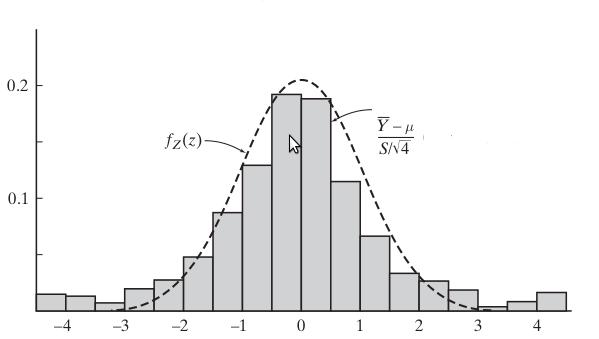
\includegraphics[height=5cm]{t1.png}

Ustteki histogram $S$ kullanarak hesaplanmistir, $n=4$ olmak uzere 500
orneklem uzerinden hesap yapilmistir. Iki dagilimin birbirinden uzaklastigi
goruluyor. 

Turetmek 

Genel olarak olasilik dagilimlari iki buyuk kategori altina duser. Asagi
yukari bir duzine kadari gercek dunyadan alinabilecek her olcumu oldugu
haliyle iyi modelleme kabiliyetine sahiptir; mesela normal, binom, Poisson,
ustel dagilimlar gibi. Diger yandan daha az sayida (ama bir o kadar onemli)
dagilimlar $n$ tane rasgele degiskenin uzerinden hesaplanan {\em
  fonksiyonlarin} nasil davrandigini cok iyi modeller. Iste bu dagilimlara
orneklem dagilimlari ismi verilir ve tipik kullanim alanlari cikarsama
(inference) yapmaktir. 

Normal dagilimi her iki kategoriye de aittir. Hem ayri ayri olcumleri
modellemek, hem de $T = \frac{\bar{Y}-\mu}{\sigma / \sqrt{n}}$'in
olasiliksal davranisini modellemek icin kullanilir. Ikinci kullanimi normal
dagilimin bir orneklem dagilimi olarak kullanilmasina ornektir. 

Normal dagilimdan sonra en onemli uc orneklem dagilimi Ogrenci t Dagilimi,
chi kare dagilimi ve F dagilimidir. Son iki dagilim t oranini temsil eden
$f_T(t)$'yi, yani $T = \frac{\bar{Y}-\mu}{\sigma / \sqrt{n}}$'yi turetmek icin gerekli.

$\chi^2$ Dagilimi

$X$, $p$ derece serbestlige sahip bir $\chi^2$ dagilima sahip ise, ki $X \sim
\chi^2_p$ olarak 
gosterilir, yogunluk 

$$ f(x) = \frac{ 1}{\Gamma(\frac{p}{2}) 2^{p/2}} x^{(p/2) - 1} e^{-x/2 }, \ x > 0 $$

formulune esittir. Bu bir teoridir ve ispatlanabilir.

Tanim

$Z_1, .. , Z_p$ bagimsiz standart Normal rasgele degiskenler ise, $\sum _{
  i=1}^{p} Z_p^2 \sim \chi^2_p$ 
esitligi dogrudur, ki bu dagilima $p$ derecede serbestlige (degrees of
freedom) olan chi kare dagilimi ismi verilir.

Teori

$Y_1,..,Y_n$ ortalamasi $\mu$, varyansi $\sigma^2$ olan bir normal
dagilimdan alinan $n$ orneklem olsun. O zaman 

a. $S^2$ ve $\bar{Y}$ birbirinden bagimsizdir

b. $\frac{(n-1)S^2}{\sigma^2} =
\frac{1}{\sigma^2}\sum_{i=1}^{n}(Y_i-\bar{Y})^2)$ hesabi $n-1$ derece
serbestligike sahip bir chi kare dagilimidir.

Ispati icin [1]'e bakiniz.

Tanim

$Z$ bir standart normal rasgele degisken, $U$ ise $n$ derece serbestlikteki
bir chi kare rasgele degisken olsun. O zaman $n$ derece serbestligi olan
Ogrenci t orani (Student's t ratio)

$$ T_n = \frac{Z}{\sqrt{ \frac{U}{n}}} $$

olarak belirtilir.

t Dagilimi (Student's t) ve Cauchy Dagilimi 

$X$, $n$ derece bagimsizlikta $t$ dagilimina sahiptir, ve dagilimi

$$ 
f_T(t) = 
\frac
{
\Gamma(\frac{n+1}{2})
}
{
\sqrt{n\pi}\Gamma(\frac{n}{2})
\bigg(1+\frac{t^2}{n}\bigg)^{(n+1)/2}
}
 $$

Aslinda Normal dagilimi $t$ dagiliminin $v = \infty$ oldugu hale tekabul
eder. Cauchy dagilimi da $t$'nin ozel bir halidir, $n = 1$ halidir. Bu
durumda yogunluk fonksiyonu

$$ f(x)  = \frac{ 1}{\pi(1+ x^2)} $$

Bu formul hakikaten bir yogunluk mudur? Kontrol icin entegralini alalim, 

$$ \int _{ -\infty}^{\infty} f(x) dx = 
\frac{ 1}{\pi} \int _{ -\infty}^{\infty} \frac{ dx}{1 + x^2} 
 $$

Cogunlukla entegre edilen yerde  ``1 arti ya da eksi bir seyin karesi''
turunde  bir ifade gorulurse, yerine gecirme (subsitution) islemi
trigonometrik  olarak  yapilir. 

$$  x = \tan \theta, \theta = \arctan x $$

$$ 1 + x^2 = 1 + \tan^2\theta = \sec^2\theta$$

$$ dx / d\theta = \sec^2\theta $$

O zaman 

$$ =
\frac{ 1}{\pi} \int _{ -\infty}^{\infty} \frac{ dx}{1 + x^2}   =
\frac{ 1}{\pi} \int _{ -\infty}^{\infty}  \frac{ 1}{\sec^2\theta}\sec^2\theta d\theta = 
\frac{ 1}{\pi} \int _{ -\infty}^{\infty}  1 \ d\theta = 
 $$

$$ = 
\frac{ 1}{\pi} \theta | _{ -\infty}^{\infty}   = 
\frac{ 1}{\pi} [\arctan(\infty) - \arctan(-\infty)]
 $$

$$ =
\frac{ 1}{\pi} [\frac{ \pi}{2} - (-\frac{ \pi}{2}) ] = 1
 $$


Kaynaklar

Larsen, {\em Introduction to Mathematical Statistics and Its Applications}

\end{document}
